\documentclass[9pt]{beamer}

% Videos
% V1, S 1-7
% V2, S 8-18
% V3, S 18-25
% V4, S 25-37 

\setbeamersize{text margin left=6mm,text margin right=8mm}

\usetheme[progressbar=frametitle]{metropolis}

\usepackage{xcolor}



\definecolor{bluegreen}{RGB}{3, 166, 155}
\definecolor{pitchblack}{RGB}{0, 0, 0}
\definecolor{lightbeige}{RGB}{255, 251, 241}
\definecolor{mediumgray}{RGB}{183, 183, 183}
\definecolor{mygreen}{rgb}{0,0.6,0}
\definecolor{mygray}{rgb}{0.5,0.5,0.5}
\definecolor{mymauve}{rgb}{0.58,0,0.82}
\definecolor{keywords}{RGB}{255,0,90}
\definecolor{comments}{RGB}{0,0,113}
\definecolor{red}{RGB}{160,0,0}
\definecolor{green}{RGB}{0,150,0}
\definecolor{navy}{RGB}{0,0,128}




% \setbeamercolor{progress bar}{fg=green,bg=blue}
% \setbeamercolor{background canvas}{bg=pitchblack}
% \setbeamercolor{normal text}{fg=lightbeige}
% \setbeamercolor{frametitle}{bg=bluegreen, fg=mediumgray}
\setbeamercolor{background canvas}{bg=white}
\setbeamercolor{normal text}{fg=black}
\setbeamercolor{frametitle}{bg=white, fg=black}



\usepackage{appendixnumberbeamer}
\usepackage{booktabs}
\usepackage[scale=2]{ccicons}

\usepackage{pgfplots}
\usepgfplotslibrary{dateplot}

\usepackage{xspace}
\newcommand{\themename}{\textbf{\textsc{metropolis}}\xspace}

\usepackage{fancyhdr}
\usepackage[mmddyyyy,hhmmss]{datetime}

% \date{\today}
\date{}
% \date[Last Compiled:]{\today}

\author{Sambasiva Rao Gangineni, Harshad Reddy Nalla, Saeed Fathollahzadeh\\ and Kia Teymourian}
\institute{13th ACM International Conference on Distributed and Event-Based Systems - DEBS 2019}

% compiled: \today , Time: \currenttime}



% This is important to set the default font to serif.
\usefonttheme{serif} % default family is serif

% \setmainfont{Liberation Serif}

% Packages for drawing arrows.
\usepackage{tikz}
\usepgflibrary{arrows}% for more options on arrows

\usepackage{pgfplots}
\usepgfplotslibrary{dateplot}
\usepackage{xspace}
% \newcommand{\themename}{\textbf{\textsc{metropolis}}\xspace}

\usepackage{blindtext}

\usepackage{listings}

% \usepackage{color}

\usepackage{caption}
\usepackage{graphicx}



\definecolor{backgroundCol}{rgb}{.97, .97, .97}
\definecolor{commentstyleCol}{rgb}{0, 0, 80}
\definecolor{keywordstyleCol}{rgb}{0.737,0.353,0.396}
\definecolor{stringstyleCol}{rgb}{0.192,0.494,0.8}
\definecolor{NumCol}{rgb}{0.686,0.059,0.569}
\definecolor{basicstyleCol}{rgb}{0.345, 0.345, 0.345}



\lstset{ %
  language=R,                     % the language of the code
  basicstyle=\footnotesize  \ttfamily \color{basicstyleCol},       % the size of the fonts that are used for the code
  % numbers=left,                   % where to put the line-numbers
  % numberstyle=\tiny\color{gray},  % the style that is used for the line-numbers
  stepnumber=1,                   % the step between two line-numbers. If it's 1, each line
                                  % will be numbered
  numbersep=2pt,                  % how far the line-numbers are from the code
  backgroundcolor=\color{white},  % choose the background color. You must add \usepackage{color}
  showspaces=false,               % show spaces adding particular underscores
  showstringspaces=false,         % underline spaces within strings
  showtabs=false,                 % show tabs within strings adding particular underscores
  frame=single,                   % adds a frame around the code
  rulecolor=\color{black},        % if not set, the frame-color may be changed on line-breaks within not-black text (e.g. commens (green here))
  tabsize=1,                      % sets default tabsize to 2 spaces
  captionpos=b,                   % sets the caption-position to bottom
  breaklines=true,                % sets automatic line breaking
  breakatwhitespace=false,        % sets if automatic breaks should only happen at whitespace
  title=\lstname,                 % show the filename of files included with \lstinputlisting;
                                  % also try caption instead of title
  keywordstyle=\color{keywordstyleCol},      % keyword style
  commentstyle=\color{commentstyleCol},   % comment style
  stringstyle=\color{stringstyleCol},      % string literal style
  escapeinside={\%*}{*)},         % if you want to add a comment within your code
  morekeywords={*,...},            % if you want to add more keywords to the set
  belowskip=-0.8 \baselineskip
}


\usepackage{algpseudocode}
\usepackage{MnSymbol,wasysym}

\definecolor{DarkGrenen}{RGB}{0,100,0}
\definecolor{DarkOliveGreen}{RGB}{85,107,47}

\definecolor{saddlebrown}{RGB}{139,69,19}




\newcommand{\red}[1]{\textcolor{red}{#1}}
\newcommand{\blue}[1]{\textcolor{blue}{#1}}
\newcommand{\green}[1]{\textcolor{DarkGrenen}{#1}}
\newcommand{\brown}[1]{\textcolor{saddlebrown}{#1}}


\newcommand{\redb}[1]{\textcolor{red}{\textbf{\boldmath{#1}}}}
\newcommand{\blueb}[1]{\textcolor{blue}{\textbf{\boldmath{#1}}}}
\newcommand{\greenb}[1]{\textcolor{DarkGrenen}{\textbf{\boldmath{#1}}}}
\newcommand{\brownb}[1]{\textcolor{saddlebrown}{\textbf{\boldmath{#1}}}}

\usepackage{url}


\usepackage{wrapfig}

\usepackage{subcaption}


% \usepackage[parfill]{parskip}



\title[Real-Time Object Recognition from Streaming LiDAR Point Cloud Data]{Grand Challenge: Real-Time Object Recognition from Streaming LiDAR Point Cloud Data}



\begin{document}

\setbeamertemplate{itemize item}{\color{red}$\triangleright$}
\setbeamertemplate{itemize subitem}{\color{blue}$\triangleright$}
% \setbeamertemplate{footline}[page number]{}

% \defbeamertemplate*{footline}{infolines theme}
% {
%   \leavevmode%
%   \hbox{%
%   \begin{beamercolorbox}[wd=1\paperwidth,ht=0.1ex,dp=3.5ex,right]{date in
%   head/foot}%
%     	\usebeamerfont{date in head/foot}\insertshortdate{}\hspace*{2em}
% 		\insertframenumber{} / \inserttotalframenumber\hspace*{3ex} 
%   \end{beamercolorbox}}%
%   \vskip0pt%
% }




\setbeamertemplate{navigation symbols}{}

% \setlist{nosep,after=\vspace{\baselineskip}}

\maketitle





%%%%%%%%%%%%%%%%%%%%%%%%%%%%%%%%%%%%%%%%%%%%
%%%%%%%%%%%%%%%%%%%%%%%%%%%%%%%%%%%%%%%%%%%%

\begin{frame}{Table of contents}
 \setbeamertemplate{section in toc}[sections numbered]
   \tableofcontents[hideallsubsections]
 
 
\end{frame}





%%%%%%%%%%%%%%%%%%%%%%%%%%%%%%%%%%%%%%%%%%%%
%%%%%%%%%%%%%%%%%%%%%%%%%%%%%%%%%%%%%%%%%%%%

\section{Paper Idea}



%%%%%%%%%%%%%%%%%%%%%%%%%%%%%%%%%%%%%%%%%%%%
%%%%%%%%%%%%%%%%%%%%%%%%%%%%%%%%%%%%%%%%%%%%



%%%%%%%%%%%%%%%%%%%%%%%%%%%%%%%%%%%%%%%%%%%%
%%%%%%%%%%%%%%%%%%%%%%%%%%%%%%%%%%%%%%%%%%%%

\begin{frame}[fragile]{Introduction}

\redb{Problems:}
\begin{itemize}
  \item test \blueb{test}   
  \item test \redb{test}   
  \item test \brownb{test}   
\end{itemize}
\end{frame}

%%%%%%%%%%%%%%%%%%%%%%%%%%%%%%%%%%%%%%%%%%%%
%%%%%%%%%%%%%%%%%%%%%%%%%%%%%%%%%%%%%%%%%%%%

\begin{frame}[fragile]{Architecture}
\redb{Steps for data processing:}
\begin{itemize}
	\item \blueb{Step 1:} Data Filtering  
	\item \blueb{Step 2:} Object Segmentation
	\item \blueb{Step 3:} Object Classification   
\end{itemize}

\begin{figure}
	\centering
	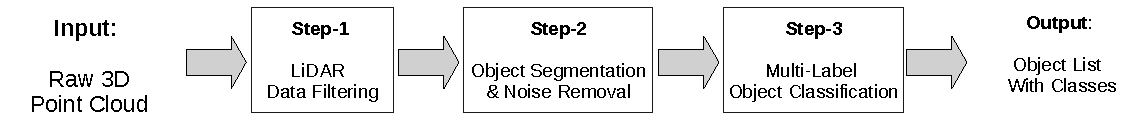
\includegraphics[width=\textwidth]{images/DataProcessingPipleline.pdf}

\end{figure}
\end{frame}


%%%%%%%%%%%%%%%%%%%%%%%%%%%%%%%%%%%%%%%%%%%%
%%%%%%%%%%%%%%%%%%%%%%%%%%%%%%%%%%%%%%%%%%%%

\begin{frame}[fragile]{Step 1: LiDAR Laser Line Data Filtering}
	\redb{Steps for Data Filtering}

\end{frame}

%%%%%%%%%%%%%%%%%%%%%%%%%%%%%%%%%%%%%%%%%%%%
%%%%%%%%%%%%%%%%%%%%%%%%%%%%%%%%%%%%%%%%%%%%

\begin{frame}[fragile]{Step 2: Object Segmentation and Noise Removal}
	\begin{itemize}
		\item segment the point cloud to chunks of data 
		
		
		\redb{3D to 2D Projection:} projected the 3D data in 4 different ways to a 2D plane and reduced the data dimensionality
		
		\begin{align*}
		d  & = \text{Distance to a projection plane} \\
		x' & =  x (\frac{d}{z}) \ \  , \ \  y' =  y (\frac{d}{z}) \ \  , \ \  z'=  z (\frac{d}{z}) = d
		\end{align*}
		
		
		\item different clustering methods to cluster the data		
		\begin{enumerate}
			\item \textbf{K-means and Mini Batch K-means} on the 3D and project 2D data.
			\item \textbf{Meanshift} on 3D and 2D data
			\item \textbf{DBSCAN} on 3D and 2D
		\end{enumerate}
	\end{itemize}
\end{frame}

%%%%%%%%%%%%%%%%%%%%%%%%%%%%%%%%%%%%%%%%%%%%
%%%%%%%%%%%%%%%%%%%%%%%%%%%%%%%%%%%%%%%%%%%%

\begin{frame}[fragile]{Step 3: Multi-class Object Classification}	
	Used for classification of point cloud data Convolutional Neural Network (CNN) 
	
	\redb{The convolutional layers:}
	\begin{itemize}
		\item Max Pooling layer
		\item Dropout Layer
		\item Fully Connected Layer  
	\end{itemize}
	
	\begin{figure}
		\centering
		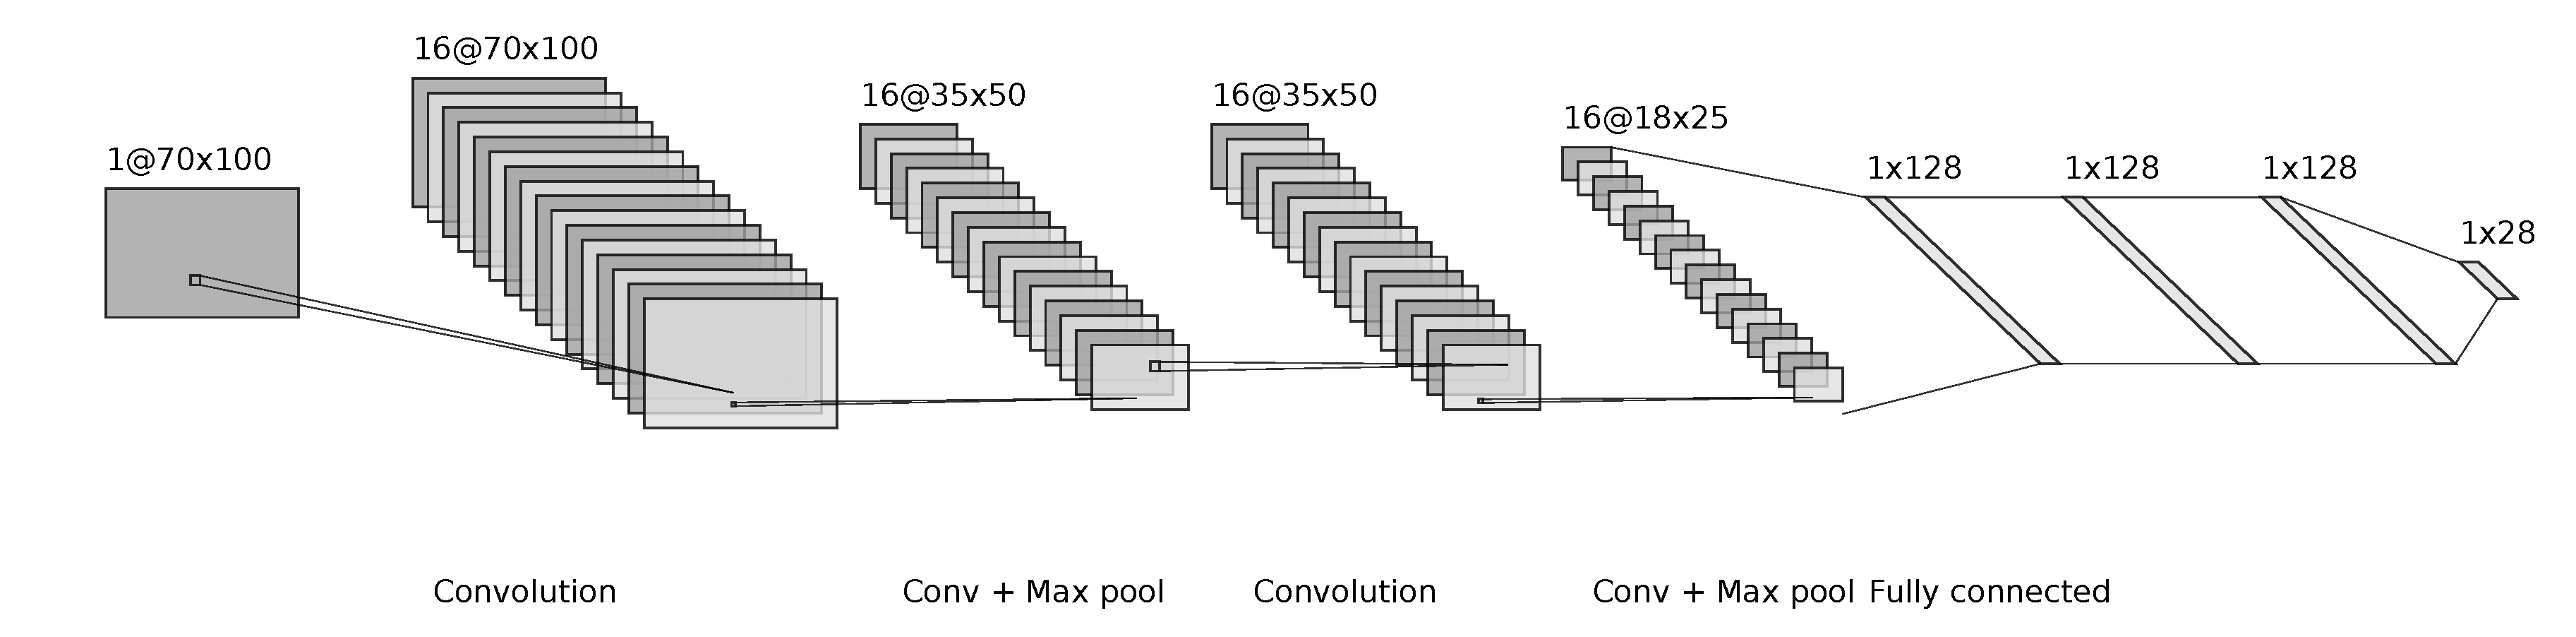
\includegraphics[width=\textwidth]{images/object_net.pdf}
		
	\end{figure}
\end{frame}

%%%%%%%%%%%%%%%%%%%%%%%%%%%%%%%%%%%%%%%%%%%%
%%%%%%%%%%%%%%%%%%%%%%%%%%%%%%%%%%%%%%%%%%%%

\begin{frame}[fragile]{Text Descriptions and Visualizations}

\redb{Two Challenges:}

\begin{enumerate}
  \item Text descriptions and interpretations  
  \item Visualizations    
\end{enumerate}


\redb{We Separated the assignments into two parts}

\begin{enumerate}
  \item Matching numbers (done by system)
  \item Correction of text description and visualizations (done by instructors/TAs) 
\end{enumerate}
 


\end{frame}


%%%%%%%%%%%%%%%%%%%%%%%%%%%%%%%%%%%%%%%%%%%%
%%%%%%%%%%%%%%%%%%%%%%%%%%%%%%%%%%%%%%%%%%%%


\section{Potential Extensions}



%%%%%%%%%%%%%%%%%%%%%%%%%%%%%%%%%%%%%%%%%%%%
%%%%%%%%%%%%%%%%%%%%%%%%%%%%%%%%%%%%%%%%%%%%

\begin{frame}[fragile]{Other Courses }

Data Science courses 

\begin{itemize}

  \item Data Mining, Machine Learning, Databases, Math, Stats   
\end{itemize}


\redb{Big Data Course} 

\begin{itemize}
  \item Each Student gets 10 GB of Data 
  \item Running on Cluster of Machines  
\end{itemize}
 
 \blueb{Solution:} Combining data partitions and pre-compute results based on combinations.  
 


\end{frame}


%%%%%%%%%%%%%%%%%%%%%%%%%%%%%%%%%%%%%%%%%%%%
%%%%%%%%%%%%%%%%%%%%%%%%%%%%%%%%%%%%%%%%%%%%
\section{System Demonstration}


%%%%%%%%%%%%%%%%%%%%%%%%%%%%%%%%%%%%%%%%%%%%
%%%%%%%%%%%%%%%%%%%%%%%%%%%%%%%%%%%%%%%%%%%%

\begin{frame}[fragile]{}

\centering
\Huge 
Thank you!

\end{frame}




\end{document}
